\clearpage
\newpage % 开始新的一页
    \thispagestyle{empty} % 移除本页的页眉和页脚[8,9](@ref)
    \newgeometry{margin=0pt} % 临时将本页的页边距全部设置为0[1](@ref)
    \noindent % 防止缩进
    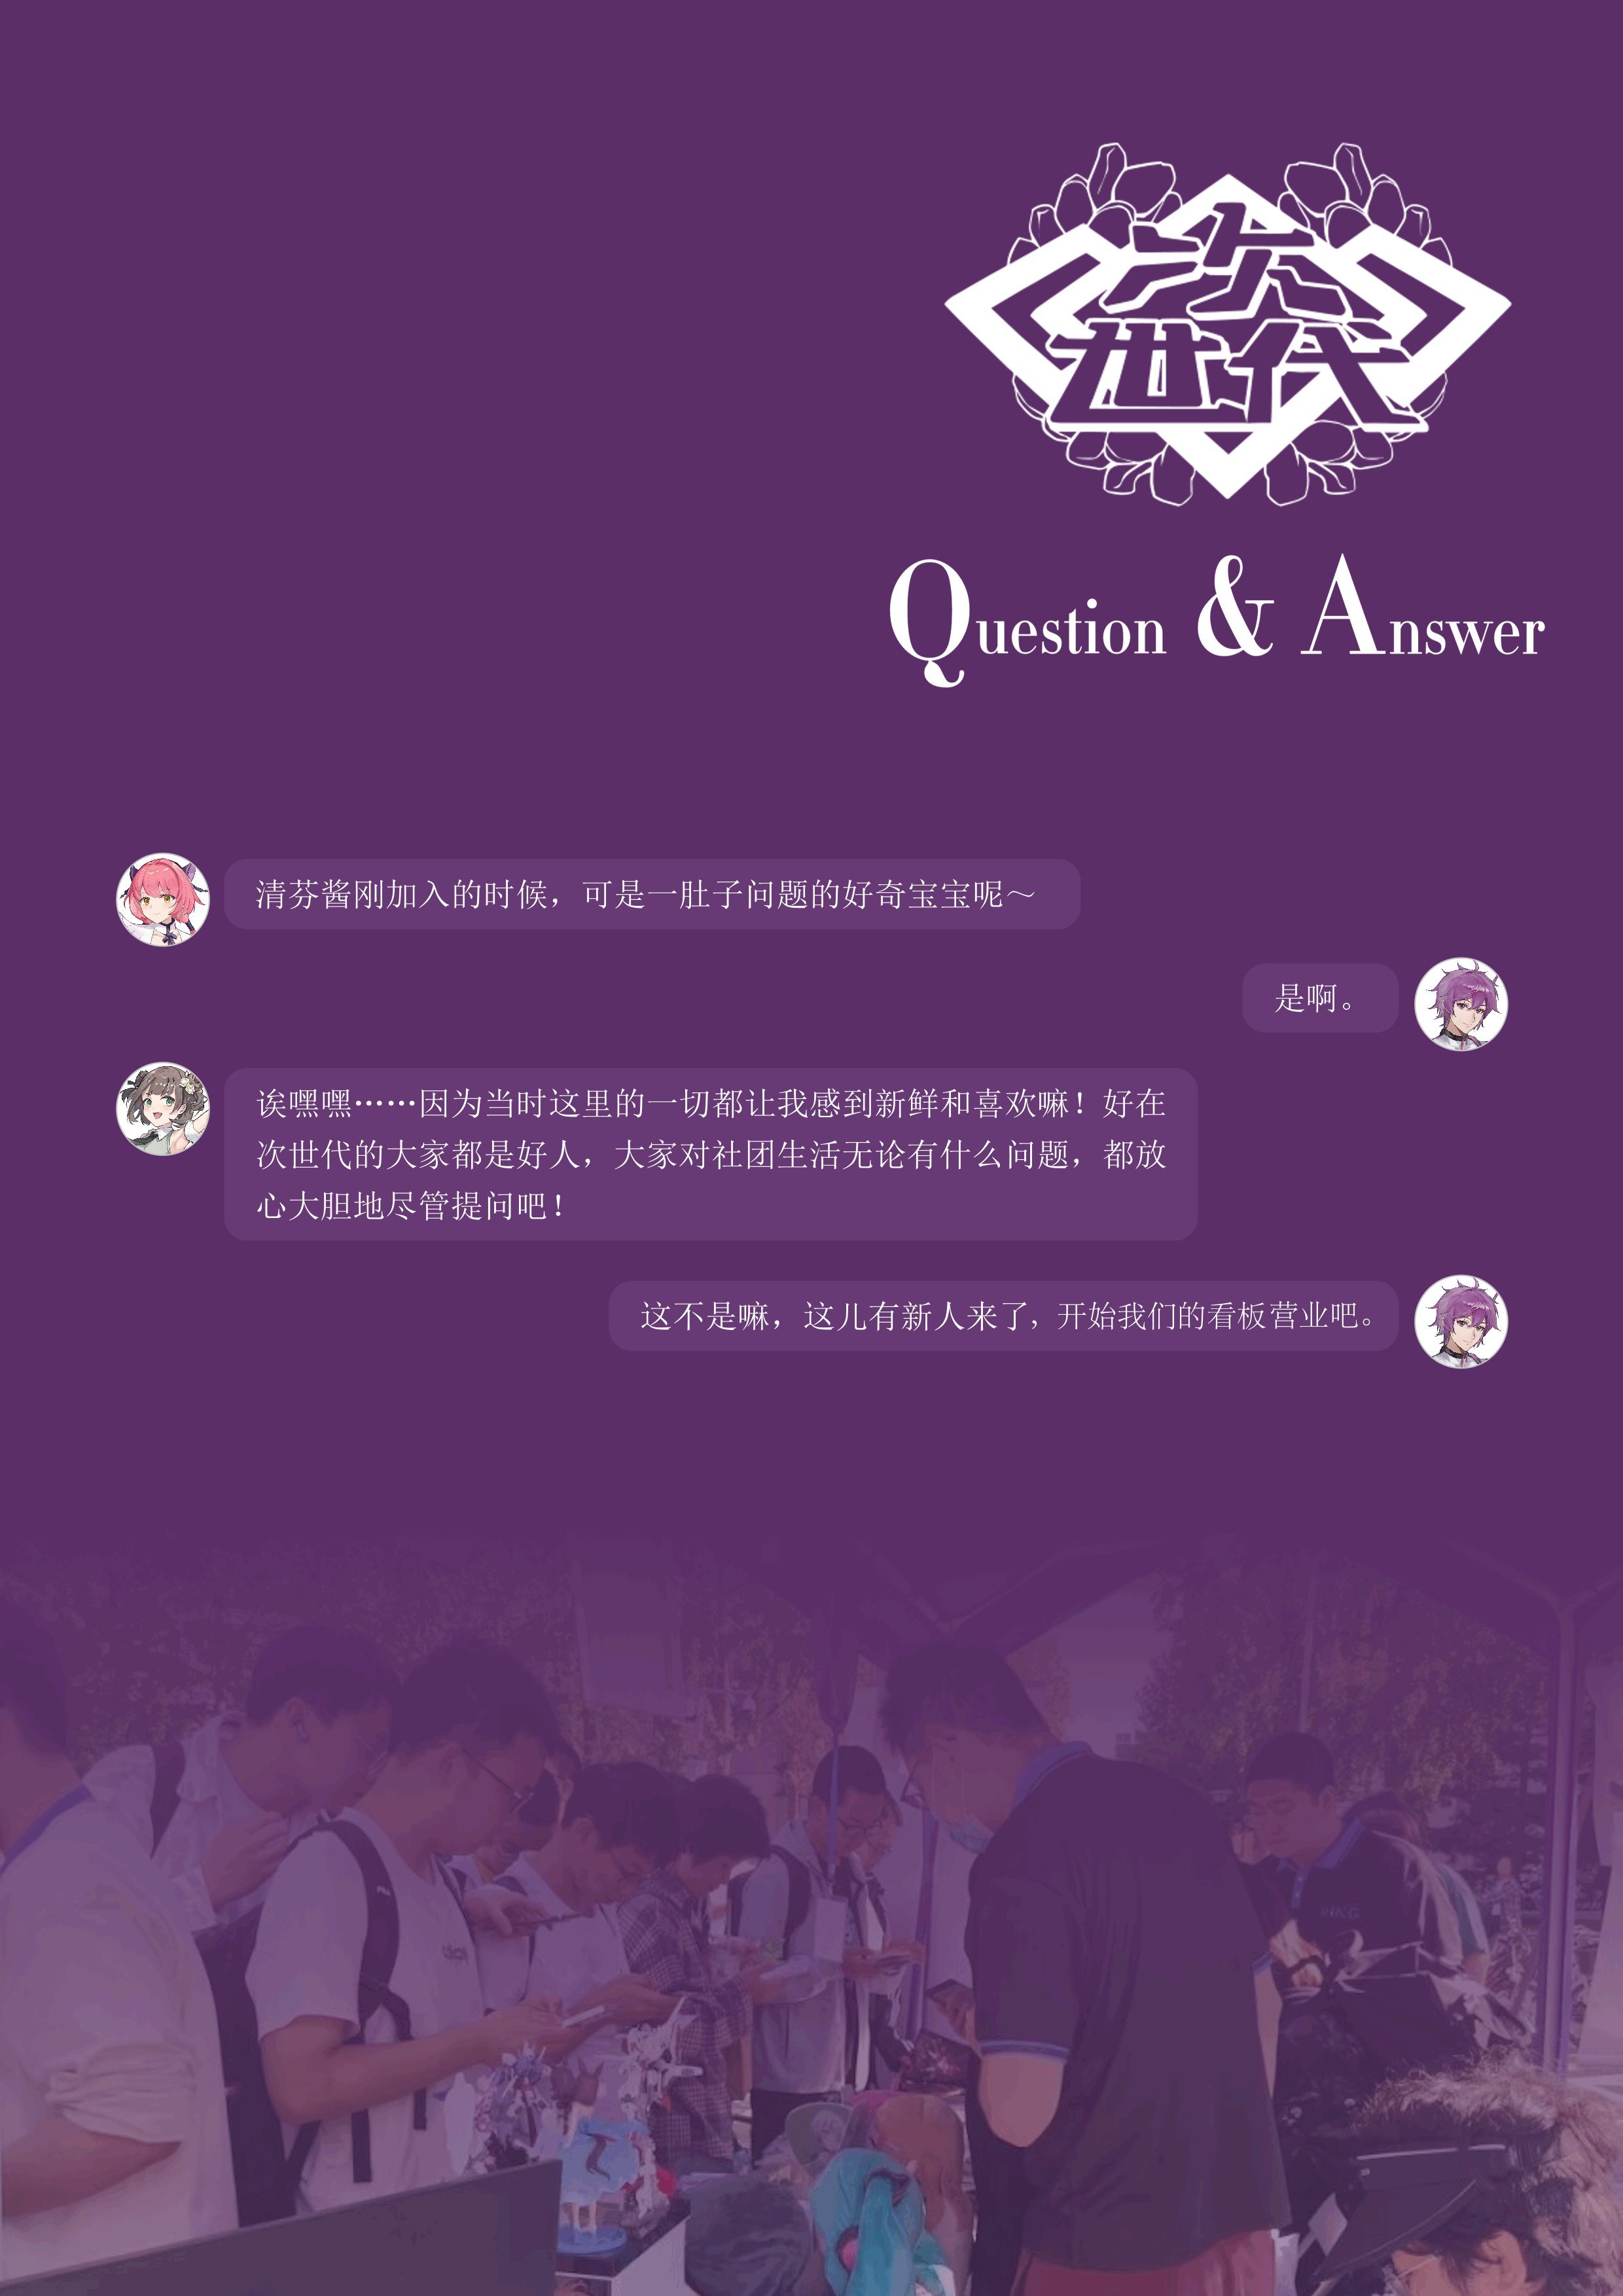
\includegraphics[width=0.9999\paperwidth, height=0.9999\paperheight]{ch3.jpg} % 插入图片,使其尺寸与纸张大小一致并保持宽高比[1](@ref)
    \restoregeometry % 恢复原来的页边距设置
\normalsize
\chatbubble[left]{qiya.jpg}{奇犽}{
 次世代有哪些活动?
}{default}

\chatbubble[right]{taozi.jpg}{桃子没有在摸鱼}{
 次世代的活动真的超级多!常驻活动有每年一次的社庆晚会,每学期一次主题咖啡厅、
 乐队live、宅舞专场演出,以及各分部自发组织的活动,如绘画部的茶绘、动研部的新番研讨会、
 地下live部的应援例会、东方部的东方例会、Lolita部的茶话会、各个二游部的集体赌博
 (给赌博来个划掉的效果)抽卡等等;此外还会不定期掉落一些大牛的讲座分享
 (已经建设过丁丁框大大和匹诺曹大大了!)、圣诞例会、配音演员见面会等等。
 未来还会有更多的活动需要由你们来建设,快来和桃子一起搞波大的吧!
}{tao}

\chatbubble[left]{guitarhero.jpg}{吉他英雄}{
  加入动漫社……是不是意味着要参加好多好多线下活动?要自我介绍?要上舞台?
  这个绝对做做做做做做做做不到!
}{default}

% 右侧聊天(用户B)
\chatbubble[right]{qingfen.jpg}{清芬哒哟}{
 绝对没这回事~我们所有的活动都是自愿参加的!当然,我们欢
 迎每一位社员的热情。但是就算只是来咖啡厅买一杯特调,来社庆做
 一枚静静的观众,或在群聊里默
 默收集好看的图片也都没问题!我们的宗旨就是玩得开心~
}{qing}

\chatbubble[left]{zijing.jpg}{紫荆(四肢驯服中)}{
 不会跳舞可以加入宅舞部吗。?
}{zi}

\chatbubble[right]{taozi.jpg}{桃子没有在摸鱼}{
 当然可以!宅舞部很多都是0基础的朋友噢~只要热爱就可以加入,
 大家会一起学舞一起练习的(抱大腿)喜欢您来!
}{tao}

\chatbubble[left]{mortis.jpg}{若叶睦(Mortis 版)}{
 想加入创作部门,但无论乐队还是绘画、cosplay、宅舞,全~都不会!
}{default}

\chatbubble[right]{qingfen.jpg}{清芬哒哟}{
 没关系,大部分人都和你一样!正是因此,几乎每个创作部门招新时都会强调:
 我们部门从不拒绝零基础选手,我们有热心太太组成的资深团队,帮助每个虚心求教的萌新快速入门!
}{qing}

\newpage

\chatbubble[left]{konami.jpg}{(该用户未填写昵称)}{
 我的品味小众又独特,该如何在次世代找到同好呢?
}{default}

\chatbubble[right]{taozi.jpg}{桃子没有在摸鱼}{
 次世代最不缺的就是小众作品爱好者(此处应有一张部门全表),只要多水群,找不到同好比找到同好还难呢!
 此外,我们秉承“三人成部”传统,只要再有两位同好,就可以申请成立一个新部门~如果你有感兴趣的领域
 还没有部门,欢迎来找我们哦!
}{tao}

\chatbubble[left]{shishangyou.jpg}{冻鳗领域大神}{
 如何向大家推荐我喜欢的作品?
}{default}

\chatbubble[right]{zijing.jpg}{紫荆}{
 有很多种方式。次世代动画研究会(简称动研部)会定期举办新番研讨会,这是安利作品、分享见解的最好机会。
 此外,次世代放映组每周都会组织放映会,现在加入放映部,完成登记和教室预约后,就可以申请放映自己喜欢的作品了。
}{zi}

\chatbubble[left]{wohenhaoqi.jpg}{好奇宝宝}{
 我也想为次世代的活动出一份力,我该如何成为帕鲁?
}{default}

\chatbubble[right]{qingfen.jpg}{清芬哒哟}{
 次世代组织部欢迎你的加入!组织部每周都会举办例会,分配下一周的工作任务。
 值得一提的是,所有任务都是自愿接受的,例会只来旁听也完全没问题~
 在主题咖啡厅、社庆等大型活动前,组织部群里还会发布志愿者招募公告,填写问卷后就可以成为帕鲁啦!
 大型活动的帕鲁可能还会有神秘福利哦~
}{qing}

\chatbubble[left]{rika.jpg}{极东魔术昼寝结社の夏社长}{
 次世代会和其他社团合作举办活动吗?
}{default}

\chatbubble[right]{zijing.jpg}{紫荆}{
 时常会有。次世代放映部不时会和学生科幻协会合作举办科幻电影放映会;主题咖啡厅也是外社
 联动的常客,荷月玩偶社、学生科幻协会等都曾是我们的联动对象。此外,学生电子音乐协会、学生推理协会
 也曾和我们有过合作。如果有任何想要进行外社联动的想法,欢迎联络组织部。
}{zi}